

\section{相対位置推定}


次に,複数のスマートデバイスの空間分布をどう推定するかについて述べる.
次のように定式化し誤差関数を最小化する最適化問題を考える.

$$
\varepsilon(\hat{x_1}, \dots, \hat{x_N}) = \sum_{i=1}^N \sum_{j\in M(i)} \left( \| \hat{ x_i } - \hat{ x_j } \| - d_{ij} \right)^2 \\
%\DeclareMathOperator*{\argmin}{arg\,min}
(\hat{x_1} \dots \hat{x_N}) = \mathrm{argmin} \varepsilon(\hat{x_1} \dots \hat{x_N})
$$

ここで,
$N \in \mathbb{N}$ は端末の数,
$M(i) \subset \{1,\dots,N\}$ は端末 $i$ と相対距離が計測できた端末の集合,
$d_{ij} \in \mathbb{R}$ は実際に計測された端末の距離とし,
$\hat{ x_i } \in \mathbb{R}^2$ n番目の端末の位置推定値で,初期値は乱数を置く.

最急降下法を使って反復的に解く.更新式は次のようになる.

$$\begin{aligned}
\hat{x_i} (n + 1) & = \left. \hat{x_i} (n) - a \frac{\partial \varepsilon}{\partial \hat{x_i}} \right|_{\hat{x} = \hat{x}(n)} \\
\frac{\partial \varepsilon}{\partial \hat{x_i}}
&= \sum_{j\in M(i)} \frac{\partial \left( \|\hat{ x_i } - \hat{ x_j }\| - d_{ij} \right)^2}{\partial \hat{x_i}} \notag\\
&= 2 \sum_{j\in M(i)} \left( \| \hat{x_i} - \hat{x_j} \| - d_{ij} \right) \frac{\partial \| \hat{x_i} - \hat{x_j} \|}{\partial \hat{x_i}} \notag\\
&= 2 \sum_{j\in M(i)} \left( 1 - \frac{d_{ij}}{\| \hat{x_i} - \hat{x_j} \|} \right) \left( \hat{x_i} - \hat{x_j} \right).
\end{aligned}$$

$n$ は反復回数, $a$ は更新式のステップ幅である.
図\ref{fig:relpo_s}にすべての端末間で距離が取得できたとしたシミュレーション結果を示す.


\begin{figure}[p]\centering
  \hspace{-2mm}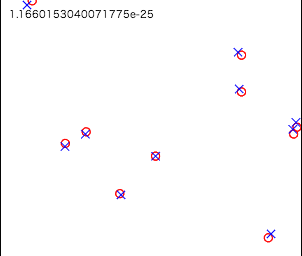
\includegraphics[clip,width=1.1\hsize]{img/positiondetection-new.png}
  \caption{最急降下法によって相対位置を解いたシミュレーション結果}\label{fig:relpo_s}
\end{figure}

端末 $i$ が測距できた他の端末の集合 $M(i)$ は後述する信号検出により決まる.
